\documentclass[a4paper,draft,12pt]{article}

\usepackage{times}
\usepackage{url}
\usepackage{hyperref}
\usepackage{float}
\usepackage{acronym}
\usepackage{paralist}
\usepackage{graphicx}
\usepackage{listings}
\usepackage{acronym}
\usepackage{pdfpages}
\usepackage{mdwlist}
\usepackage[margin=2cm]{geometry}

\acrodef{CAS}{compare-and-swap}

\lstset{ %
    breaklines=true,
    basicstyle=\footnotesize,
    moredelim=[is][\bfseries]{[*}{*]}
}

% ----------------------------------------------------------------------------
% Start the document
%

\title{\textbf{A Java implementation of \\Non-blocking Binary Search Trees}} % Article title

\author{
    \textsc{Alessio Bogon}\\[2mm] % Your name
    \normalsize University of Trento - Master Degree in Computer Science\\ % Your institution
    \normalsize Concurrency\\
    \href{mailto:alessio.bogon@studenti.unitn.it}{alessio.bogon@studenti.unitn.it} % Your email address
}
\date{\today}

\begin{document}

\maketitle

% - In REPORT describe the main difficulties you encountered, how you solved
% them, and explain informally why you believe it works

\section{Introduction} %(fold)
\label{sec:introduction}
This project is a non-blocking concurrent Java implementation of the binary search tree structure, and aims to reproduce the work of Ellen et al\cite{ellen10}.
The basic interface that we target is the \texttt{Set<T>}, with the \emph{find}, \emph{insert} and \emph{remove} operations.
The class that implements it is \texttt{Non\-Blocking\-Binary\-Search\-Tree\-<T>}, inside the \texttt{it.unitn.studenti.alessiobogon.concurrency.nbbst} package.

All the interface methods implemented are total and lock-free. Moreover, the \texttt{find} method is wait-free.
This is due to the fact that insertions and deletions might need to \emph{help} other ongoing operations in order to complete, while \texttt{find} can just look for the item without caring since the tree is always in a consistent state.

The project also provides the following features:
\begin{itemize*}
    \item \textbf{Java ``generics''} When useful, classes are declared using generic types.
    \item \textbf{Javadoc} Classes documentation.
    \item \textbf{OCaml-like output syntax} Tree representation in OCaml-like style.
    \item \textbf{Dot output syntax} Tree representation in the ``dot'' format.
    \item \textbf{Logging facility} The class logs all the important events. You can choose to print just method calls/returns or to go deeper and show also the result of CAS operations.
\end{itemize*}

% section introduction (end)

\section{Usage} % (fold)
\label{sec:usage}
The program can be executed by running the provided script on UNIX platforms:
\begin{verbatim}
    ./run.sh
\end{verbatim}
It basically compiles all the sources needed by the main class and then run it.
Please ensure that you are using Java 7 or above and that the \texttt{java} and \texttt{javac} executables are available in your \texttt{PATH}.
You can also configure the verbosity level of the output via the VM parameters (e.g. \texttt{java -DlogLevel=FINEST ...}), which allows to trace the various \ac{CAS} operations.
The default level is \emph{FINE}, which shows the methods invocations and return values of the interface methods.
The main class will also save the dot representation of the resulting graph inside the \texttt{graph.dot} file.
Please refer to \texttt{README.txt} for further information.

The provided Main class uses five threads and executes many operations, but for the sake of brevity we report this simple history, where three threads tries to do the operations described in Table~\ref{table:thread_ops}.

\begin{table}
\centering
\begin{tabular}{c|c|c}
{\bf Thread\#10} & {\bf Thread\#11} & {\bf Thread\#12} \\
\hline
\texttt{bst.insert(20)}   & \texttt{bst.insert(15)}   & \texttt{bst.insert(30)}   \\
\texttt{bst.insert(30)}   & \texttt{bst.delete(20)}   & \texttt{bst.find(20)}     \\
                 & \texttt{bst.find(15)}     & \texttt{bst.insert(15)}   \\
                 &                  & \texttt{bst.find(20)}
\end{tabular}
\caption{Threads operation example}
\label{table:thread_ops}
\end{table}

One possible execution is the following:
\begin{verbatim}
[02:03:55.648] Thread#10:    insert: ENTRY 20
[02:03:55.648] Thread#12:        insert: ENTRY 30
[02:03:55.648] Thread#11:      insert: ENTRY 15
[02:03:55.652] Thread#10:    insert: RETURN true
[02:03:55.653] Thread#10:    insert: ENTRY 30
[02:03:55.653] Thread#10:    insert: RETURN true
[02:03:55.654] Thread#11:      insert: RETURN true
[02:03:55.654] Thread#11:      delete: ENTRY 20
[02:03:55.655] Thread#12:        insert: RETURN false
[02:03:55.655] Thread#12:        find: ENTRY 20
[02:03:55.655] Thread#12:        find: RETURN true
[02:03:55.655] Thread#12:        insert: ENTRY 15
[02:03:55.656] Thread#12:        insert: RETURN false
[02:03:55.656] Thread#11:      delete: RETURN true
[02:03:55.656] Thread#12:        find: ENTRY 20
[02:03:55.656] Thread#11:      find: ENTRY 15
[02:03:55.657] Thread#12:        find: RETURN false
[02:03:55.657] Thread#11:      find: RETURN true
The resulting tree is: Node(2147483647, Node(2147483646,
    Node(30, Leaf(15), Leaf(30)), Leaf(2147483646)),
    Leaf(2147483647))
[02:03:56.023] Thread#1:  main: Graph written into graph.dot
[...]
\end{verbatim}

As you can verify, this is a valid execution: Thread 10 and 11 successfully complete all the operations.
Thread 12 fails to insert 30 because it already exists, then it finds 20 because Thread 10 inserted it before (and Thread 11 didn't delete it yet), then it fails again trying to insert 15 and then it looks for 20 and can't find it since Thread 11 managed to delete it.
You can see the resulting tree in the output and in the file \texttt{graph.dot}.
Fig.~\ref{fig:test} shows the output for this execution.

\begin{figure}
    \centering
    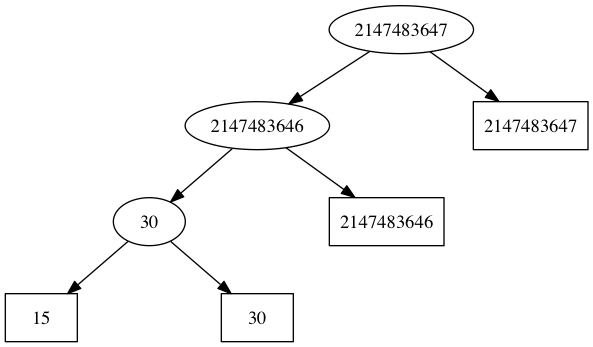
\includegraphics[width=0.7\textwidth]{test}
    \caption{
    Visualization of the output tree for the example given in Section~\ref{sec:usage}.
    Internal nodes are represented by ellipses, while leafs are represented by boxes.
    The top two nodes are $\infty_2$ and $\infty_1$ respectively.
    }
    \label{fig:test}
\end{figure}

\section{Implementation}
The provided implementation is basically a rewriting of the work done by Ellen et al in Java.
Some trickery is needed when dealing with the \ac{CAS} objects.

The types described in the paper (\emph{Update}, \emph{Internal}, \emph{Info}, etc.) are implemented using classes, according to the standard OOP paradigms (subclassing, abstract classes, etc.).
All the fields that are not mutable are declared using the \emph{final} modifier, to ensure they do not change (e.g., \texttt{key} field of nodes).

The \texttt{Non\-Blocking\-Binary\-Search\-Tree<T>} class implements the algorithms described in the paper and its state is given by a reference to the root node.
The following is a brief overview of the most interesting methods:
\begin{itemize}
    \item \texttt{find(T item)}: it descends the tree looking for the element with key given by the hash code of the item.
    It returns true if and only if it has been found.
    This function is wait-free, since it does not help ongoing operations.
    \item \texttt{insert(T item)}: it looks for the parent of the new node to insert, after checking that it is not already present.
    Then it creates an \texttt{UpdateInfo} object with all the information required to complete this operation.
    It tries to \emph{iflag} the parent, and if the operation was successful it physically adds the new node (\emph{ichild}) and marks the parent as clean (\emph{iunchild}).
    If it was not possible to \emph{iflag} the parent, then it starts the procedure again.
    This function is lock-free, because it might encounter some unfinished operations that prevents the insertion, and in that case it would help them to complete.
    \item \texttt{remove(T item)}: it looks for the parent and the grandparent of the node to remove, if any.
    Just like the previous method, it creates a \texttt{DeleteInfo} object with enough information for any thread to complete the deletion.
    Then it tries to \emph{dflag} the grandparent node: if it fails, it starts the procedure again, if it succeeds then it tries to \emph{mark} the parent node.
    If it fails, it starts the procedure again, otherwise it completes the operation with the \emph{dchild} (physical node removal) and \emph{dunflag} (set grand parent state back to clean) steps.
    Also this method is lock-free, because it might need to \emph{help} other operations.
    \item \texttt{help(), helpDelete(), helpMarked(), etc.}: these methods are to be called by insertions and deletions that needs to finish an operation in order to complete.
\end{itemize}
To get a deeper view of the class, please refer to the \emph{javadoc}.

\subsection{Challenges} % (fold)
\label{ssec:challenges}

In order to achieve the \emph{non-blocking} requirements we use the Java variant of the \acf{CAS} operation, which is the compare-and-set.
The key difference is that compare-and-swap returns the value the object had before the operation, while compare-and-set returns \emph{true} if and only if the operation has been completed successfully.

In the paper, the result of a compare-and-swap operation is checked by comparing the value returned with the one we are expecting. If they are equal, this means that the operation was successful, otherwise the operation failed.
With the compare-and-set semantics, it is sufficient to check the return value to determine the outcome.

The main difficulty comes when we need to check the reason why an operation was unsuccessful.
This happens in the \texttt{helpDelete()} method: it tries to \emph{MARK} the parent node of the given operation, but the compare-and-set might fail because some other thread already marked it.
In this case we cannot blindly return false, because it would mean that the operation cannot be completed and needs to backtrack.
To solve this, the result of the compare-and-set is checked. If it failed, the current state of the parent is obtained and checked if it has been \emph{MARK}ed by another node.
This works fine because, intuitively, once a node has been marked it cannot change its state (from this point, the \texttt{delete()} operation can only succeed) and will eventually be physically deleted by unlinking it from its parent (\texttt{dchild}).

Another problem comes with the implementation of the \texttt{Node.update} field, which is a \emph{word} that points to an \texttt{Info} record. This same word is also used to store a \texttt{State} record, by stealing the first two bits. Since in Java we do not have access to raw pointers, we cannot steal the first two bits of the reference. To quote David Wheeler, ``all problems in computer science can be solved by another level of indirection [...]'': indeed the provided solution just wraps the \texttt{Info} and \texttt{State} records into an \texttt{Update} object. To conclude, the \texttt{Node.update} field is an \texttt{Atomic\-Reference} that points to an \texttt{Update} object.

Alternatively, one could have used the \texttt{AtomicStampedReference}, but this class does exactly what is described above\footnote{See the OpenJDK implementation at \url{https://github.com/openjdk-mirror/jdk7u-jdk/blob/jdk7u6-b08/src/share/classes/java/util/concurrent/atomic/AtomicStampedReference.java}}. However this would make the code less clear, so the former solution is used.

Worth of note is the fact that the paper initializes the tree with two special values, $\infty_2$ and $\infty_1$. To manage this issue this implementation replaces them with \texttt{Integer.MAX\_VALUE} and \texttt{Integer.MAX\_VALUE - 1} respectively. The only limitation is that it is not possible to insert nodes with such values, but it is an acceptable compromise in my opinion. Alternatively, one could write an \texttt{ExtendedInteger} class that implements the \texttt{Comparable} interface and that deals with these special values. This would result in a more messy code because comparisons like \texttt{this.key < other.key} would become \texttt{this.key.compareTo(other.key) == -1}, since Java does not allow to define custom operator overloads.


\begin{thebibliography}{9}
    \bibitem{ellen10} Ellen, F., Fatourou, P., Ruppert, E., and van Breugel, F. \emph{Non-blocking Binary Search Trees}. Proceedings of the 29th Annual ACM Symposium on Principles of Distributed Computing (PODC), 131–140, 2010.
\end{thebibliography}


\end{document}
